\documentclass[a4paper, 12pt]{article}


\usepackage{float}     
\usepackage{placeins} 
\usepackage{afterpage}  

\renewcommand{\topfraction}{.85}
\renewcommand{\bottomfraction}{.7}
\renewcommand{\textfraction}{.15}
\renewcommand{\floatpagefraction}{.66}
\setcounter{topnumber}{9}
\setcounter{bottomnumber}{9}
\setcounter{totalnumber}{20}

\usepackage[T1]{fontenc}
\usepackage{lmodern}
\usepackage{color}
\usepackage{amsfonts}
\usepackage{epstopdf}
\usepackage{matlab}
\usepackage{booktabs}
%\documentclass{book}
\usepackage{blindtext}
\usepackage{hyperref}
\usepackage[brazil]{babel}

\usepackage{subfig}
\usepackage{amssymb}
\usepackage[utf8]{inputenc}
\usepackage{amsmath}
\usepackage{indentfirst}
\usepackage{graphicx}
\usepackage{listings}
\usepackage{tcolorbox}
\usepackage{upgreek}
\usepackage{multicol,lipsum}
\usepackage[a4paper,
top=3cm, left=3cm, bottom=3cm, right=3cm]{geometry}
\usepackage{setspace}
\usepackage{multirow}
\usepackage{float}
\usepackage[dvipsnames]{xcolor}
\usepackage[table]{xcolor}
%\usepackage{pdflscape}
\usepackage[DIV=15]{typearea}
\usepackage[nottoc]{tocbibind}
\usepackage[sort,numbers]{natbib}
%\usepackage{cite}
\usepackage{matlab}

\usepackage[utf8]{inputenc}
\usepackage[T1]{fontenc}
\usepackage{lmodern}
\usepackage{graphicx}
\usepackage{color}
\usepackage{hyperref}
\usepackage{amsmath}
\usepackage{amsfonts}
\usepackage{epstopdf}
\usepackage[table]{xcolor}
\usepackage{matlab}

\lstdefinestyle{python}{
  language=Python,
  basicstyle=\ttfamily,
  keywordstyle=\color{blue},
  stringstyle=\color{green},
  commentstyle=\color{gray},
  numbers=left,
  numberstyle=\tiny\color{gray},
  stepnumber=1,
  numbersep=5pt,
  backgroundcolor=\color{white},
  showspaces=false,
  showstringspaces=false,
  showtabs=false,
  frame=single,
  rulecolor=\color{black},
  tabsize=4,
  captionpos=b,
  breaklines=true,
  breakatwhitespace=false,
  title=\lstname,
  escapeinside={\%*}{*)},
  morekeywords={self},
  emph={MyClass,__init__},
  emphstyle=\color{red}
}


\documentclass[letterpaper]{article}
% bib pack %%%%%%%%%%%%%%%%%%%%%%%%%%%%%%%%%%%%%%%%%%%%%%%%%%%%%%%%%%%%%%%%%%%%%
\usepackage[utf8]{inputenc}
\usepackage{geometry}
    \geometry{left=3cm,right=2cm,top=2cm,bottom=2cm}
%
\usepackage[spanish]{babel}
%
\usepackage[fixlanguage]{babelbib}
    \bibliographystyle{babunsrt}
%
\usepackage{url}

\begin{document}
%\maketitle

\begin{titlepage}
	\begin{center}
		% --- Logo e Instituição ---
		
\includegraphics[width=13cm]{images/puc-rio-logo.png}
		\vspace{0.5cm}
		
	
		
		\textsc{\large Departamento de Engenharia Elétrica}
		
		\vfill 
		
		\huge{\textbf{Laboratório de Técnicas Digitais}}
		
		\vspace{0.5cm}
		
		\Large{ENG4413}
		
		\vspace{2cm}
		
		\Large{\textbf{Relatório de Atividades 1}}
		
		\vspace{0.5cm}
		
		\large{}
		
		\vfill 
	\end{center}
	
	\begin{flushleft}
		\begin{tabbing}
		Aluno(a)\qquad\qquad\=\>Paloma Fernanda Loureiro Sette - 1621595\\
  Aluno(a)\qquad\qquad\=\>João  Dias de Miranda - 1911231\\
			Professor(a)\>Moisés Henrique Szwarcman \\
	\end{tabbing}
		  
	\end{flushleft}
	
	\vfill 
	
	% --- Local e Data ---
	\begin{center}
		\large
		Rio de Janeiro \\
		\today % Usa a data atual automaticamente
	\end{center}
\end{titlepage}
%%%%%%%%%%%%%%%%%%%%%%%%%%%%%%%%%%%%%%%%%%%%%%%%%%%%%%%%%%%
\newpage
\tableofcontents
\thispagestyle{empty}

\newpage
\pagenumbering{arabic}

\newpage

%\newcommand{\listequationsname}{Lista de Equações}
%\newlistof{myequations}{equ}{\listequationsname}
%\newcommand{\myequations}[1]{%
%\addcontentsline{equ}{myequations}{\protect\numberline{\theequation}#1}\par}

%\listofmyequations
\newpage


\newpage

\listoffigures
\thispagestyle{empty}

\newpage
%%%%%%%%%%%%%%%%%%%%%%%%%%%%%%%%%%%%%%%%%%%%%%%%%%%%%%%%%
%%%%%%%%%%%%%%%%%%%%%%%%%%%%%%%%%%%%%%%%%%%%%%%%%%%

\newpage

\thispagestyle{empty}

\newpage

\section{Introdução}

O presente relatório detalha o processo de projeto, minimização e simulação de um circuito lógico combinacional, conforme solicitado na primeira experiência de laboratório da disciplina de Técnicas Digitais. O problema proposto consiste em desenvolver um sistema digital capaz de identificar, a partir de um número de entrada de 5 bits representando 32 salas (numeradas de 0 a 31), quais delas são equipadas com projetores, sinalizando o resultado em uma saída de 1 bit.

A solução do problema baseia-se em conceitos fundamentais da eletrônica digital. Um circuito combinacional é caracterizado pelo fato de sua saída depender exclusivamente da combinação das suas entradas em um determinado instante. A relação entre as entradas e a saída é descrita por uma função booleana, que serve como a representação matemática do comportamento lógico do sistema. O objetivo principal da engenharia de circuitos digitais é encontrar a implementação física mais eficiente para essa função, o que é alcançado através de técnicas de minimização.

Para atingir o objetivo, a metodologia adotada seguiu as etapas clássicas de um projeto de lógica combinacional:
\begin{itemize}
    \item Análise da especificação do problema para identificar as variáveis de entrada e saída e derivar a tabela-verdade da função.
    \item Obtenção da expressão booleana na sua forma canônica de Soma de Produtos (SDP), utilizando os mintermos correspondentes às condições de saída "1".
    \item Minimização da expressão booleana pelo método do Mapa de Karnaugh, a fim de reduzir o número de termos e literais, resultando em um circuito com menor custo e complexidade.
    \item Simulação do circuito mínimo projetado utilizando o software CircuitMaker 2000, implementado com Circuitos Integrados (CIs) da família TTL Série 74, conforme especificado.
\end{itemize}

As seções seguintes deste relatório apresentarão o desenvolvimento teórico detalhado, incluindo a derivação da função mínima, e os resultados práticos obtidos na simulação do circuito final.


\section{Desenvolvimento Teórico}

\subsection{Análise da Especificação}
A primeira etapa do projeto foi a análise detalhada do problema proposto. O objetivo é projetar um circuito lógico combinacional mínimo, cuja entrada é o número de uma sala de um total de 32 (de 0 a 31), representado em binário. A saída do circuito deve ser "1" se a sala for equipada com projetor e "0" caso contrário. O circuito deve ser montado usando circuitos integrados (CIs) da família TTL Série 74, e simulado com chaves digitais na entrada e um LED na saída.

As salas equipadas com projetor foram especificadas como:
\begin{itemize}
    \item Salas 0, 1, 3, 9, 10, 11, 17, e 19.
    \item Todas as salas com numeração maior que 25 (ou seja, 26, 27, 28, 29, 30 e 31).
\end{itemize}

\subsection{Representação Binária e Variáveis de Entrada}
Para que um sistema digital possa processar os números das salas, eles devem ser convertidos para o formato binário, a linguagem fundamental dos circuitos. Como existem 32 salas (numeradas de 0 a 31), o desafio é representá-las usando apenas os símbolos binários "0" e "1". A solução é utilizar um número de bits (N) suficiente para cobrir todas as posições ($2^N$), o que, para 32 posições, exige 5 bits ($2^5 = 32$).

Assim, o circuito possui 5 variáveis de entrada, que foram denominadas de A, B, C, D e E. A variável A foi definida como o bit mais significativo (valendo 16), e E como o menos significativo (valendo 1). A seguir, exemplos de conversão:
\begin{itemize}
    \item Sala 0: $00000_2$ (A=0, B=0, C=0, D=0, E=0)
    \item Sala 9: $01001_2$ (A=0, B=1, C=0, D=0, E=1)
    \item Sala 26: $11010_2$ (A=1, B=1, C=0, D=1, E=0)
    \item Sala 31: $11111_2$ (A=1, B=1, C=1, D=1, E=1)
\end{itemize}

\subsection{Derivação da Função Lógica}
A função do circuito, que chamamos de P (Projetor), é acionada (saída P=1) apenas quando as entradas correspondem a uma das salas com projetor. As combinações de entrada que resultam em uma saída lógica "1" são chamadas de mintermos. A lista completa de mintermos para este problema, em ordem crescente, é:
\begin{center}
    P=1 $\rightarrow$ sala $\in$ \{0, 1, 3, 9, 10, 11, 17, 19, 26, 27, 28, 29, 30, 31\}
\end{center}
A partir desta lista, a função booleana pode ser expressa em sua forma canônica de Soma de Produtos (SDP), representando o somatório de todos os mintermos:
\begin{equation}
    P(A,B,C,D,E) = \sum m(0, 1, 3, 9, 10, 11, 17, 19, 26, 27, 28, 29, 30, 31)
\end{equation}



\subsection{Minimização por Mapa de Karnaugh}

Para simplificar a expressão canônica obtida anteriormente, utilizou-se o método do Mapa de Karnaugh (Mapa K) para 5 variáveis. Este método consiste em dois mapas de 4 variáveis, um para a condição A=0 e outro para A=1, que permitem a identificação visual de termos logicamente adjacentes para a minimização da função. Os mapas preenchidos com os mintermos da função P e os respectivos agrupamentos são mostrados na Figura \ref{fig:mapak}.


\begin{figure}[H]
    \centering

    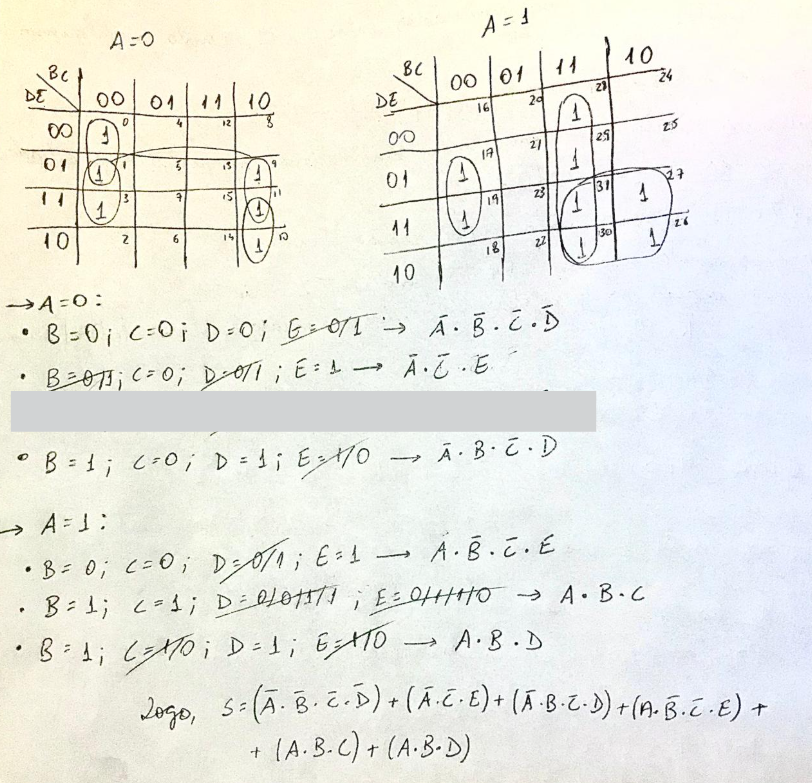
\includegraphics[width=1\textwidth]{images/mapa-k.png}
    \caption{Mapas de Karnaugh para A=0 e A=1 com os agrupamentos dos mintermos.}

    \label{fig:mapak}
\end{figure}


A análise dos agrupamentos (implicantes primos) nos mapas resultou nos seguintes termos simplificados:

\begin{enumerate}
    \item \textbf{No mapa A=0:} O agrupamento dos mintermos \{0, 1\} resulta na eliminação da variável E, gerando o termo $\overline{A} \cdot \overline{B} \cdot \overline{C} \cdot \overline{D}$.
    \item \textbf{No mapa A=0:} O agrupamento de 4 células dos mintermos \{1, 3, 9, 11\} elimina as variáveis B e D, gerando o termo $\overline{A} \cdot \overline{C} \cdot E$.
    \item \textbf{No mapa A=0:} O agrupamento dos mintermos \{10, 11\} elimina a variável E, gerando o termo $\overline{A} \cdot B \cdot \overline{C} \cdot D$.
    \item \textbf{No mapa A=1:} O agrupamento dos mintermos \{17, 19\} elimina a variável D, gerando o termo $A \cdot \overline{B} \cdot \overline{C} \cdot E$.
    \item \textbf{No mapa A=1:} O agrupamento de 4 células dos mintermos \{28, 29, 30, 31\} elimina as variáveis D e E, gerando o termo $A \cdot B \cdot C$.
    \item \textbf{No mapa A=1:} O agrupamento de 4 células dos mintermos \{26, 27, 30, 31\} elimina as variáveis C e E, gerando o termo $A \cdot B \cdot D$.
\end{enumerate}

A soma de todos os termos resultantes dos implicantes primos essenciais nos fornece a expressão booleana mínima para a função P.

\begin{equation}
P = \overline{A}.\overline{B}.\overline{C}.\overline{D} + \overline{A}.\overline{C}.E + \overline{A}.B.\overline{C}.D + A.\overline{B}.\overline{C}.E + A.B.C + A.B.D
\label{eq:expressao_minima}
\end{equation}

Esta equação (\ref{eq:expressao_minima}) é a base para a implementação do circuito lógico no simulador, pois representa a solução mais eficiente em termos de número de portas e entradas.


\section{Simulação e Resultados}

A implementação do circuito lógico minimizando foi realizada no software CircuitMaker 2000, utilizando portas lógicas da família TTL Série 74. As entradas A, B, C, D e E foram configuradas por meio de chaves digitais, enquanto a saída foi conectada a um LED indicador, representando a presença de projetor nas salas especificadas.

Durante a simulação, foram testadas todas as combinações de entrada correspondentes aos números das salas (0 a 31). Observou-se que, para as entradas que representam salas 0, 1, 3, 9, 10, 11, 17, 19, 26, 27, 28, 29, 30 e 31, o LED ascendeu corretamente, indicando saída lógica igual a 1. Para as demais combinações, a saída permaneceu em nível lógico 0, confirmando a fidelidade do circuito em relação à tabela-verdade e à função booleana minimizada.

A figura 2 abaixo apresenta a tela do simulador, onde é possível visualizar a montagem do circuito e a resposta obtida. Dessa forma, verificou-se que o projeto implementado atende integralmente às especificações propostas, com comportamento consistente em todos os casos de teste. 

\begin{figure}[H]
    \centering

    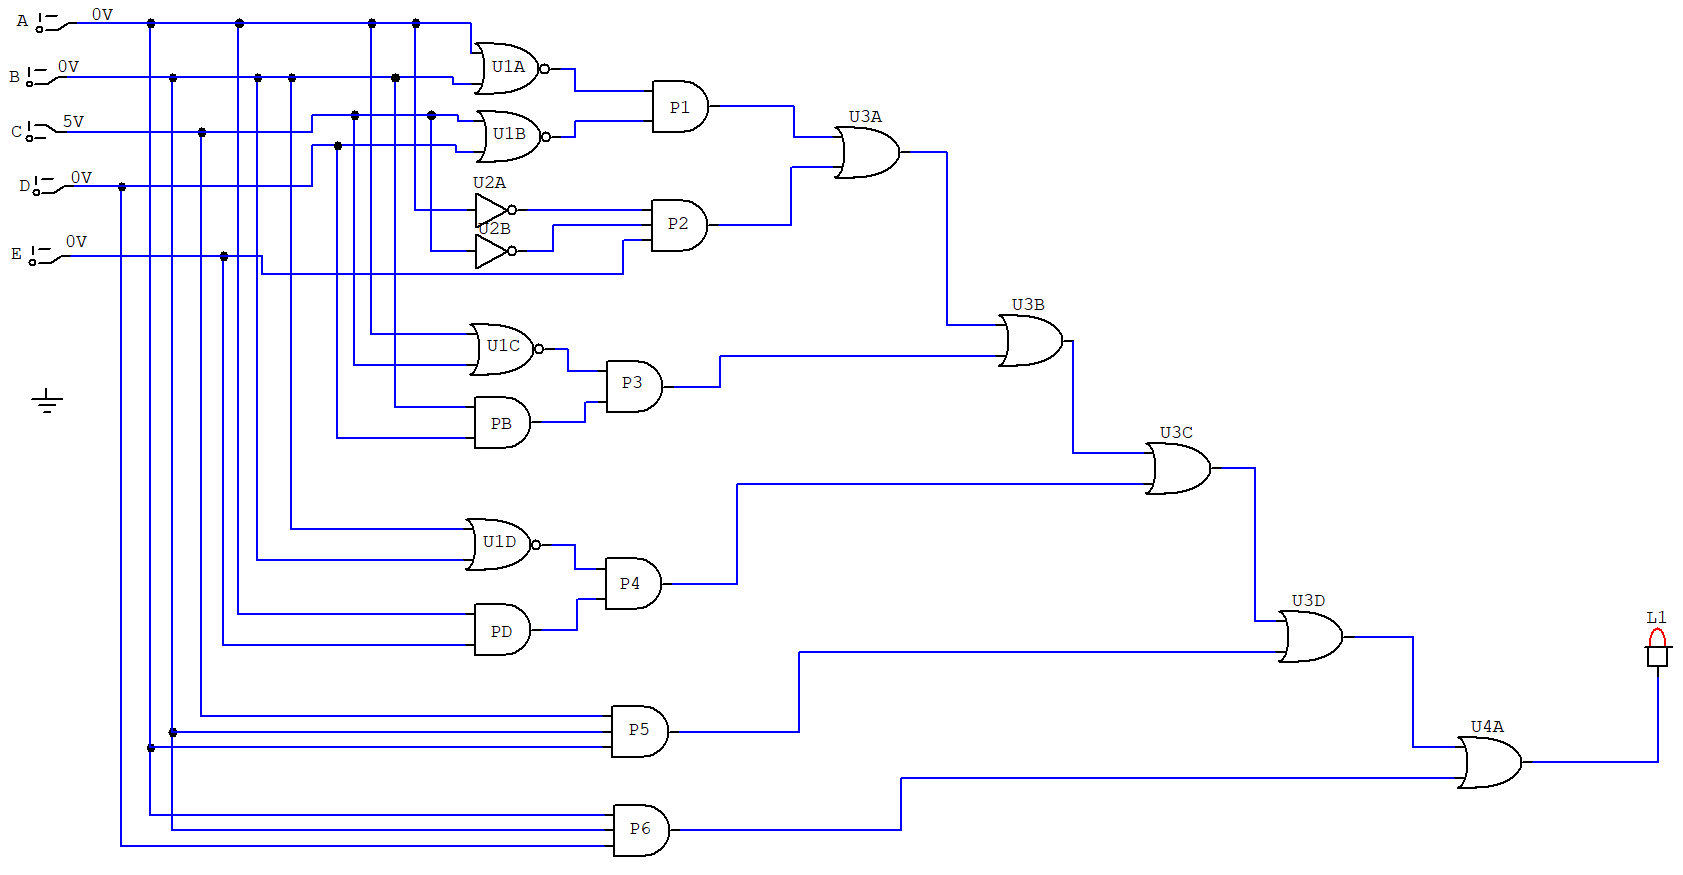
\includegraphics[width=1\textwidth]{images/simulacao.png}
    \caption{Simulação no CircuitMaker.}

    \label{fig:mapak}
\end{figure}

\section{Conclusão}

O experimento permitiu aplicar de forma prática os conceitos de simplificação e implementação de circuitos lógicos combinacionais. A partir da análise da especificação, foi possível derivar a função booleana na forma canônica, simplificá-la por meio do Mapa de Karnaugh e, em seguida, implementar a versão mínima no simulador.

Os resultados obtidos comprovam que o circuito desenvolvido é capaz de identificar corretamente as salas equipadas com projetores, utilizando uma arquitetura otimizada em número de portas lógicas. Além disso, a atividade reforçou a importância da minimização na redução de custos e complexidade do hardware, evidenciando a relação entre teoria e prática no contexto da eletrônica digital.

Conclui-se, portanto, que os objetivos do laboratório foram completamemte atingidos, proporcionando ao aluno a consolidação dos fundamentos de lógica booleana e técnicas de simulação de circuitos digitais.










% REFERENCIAS %%%%%%%%%%%%%%%%%%%%%%%%%%%%%%%%%%%%%%%%%%%%%%%%%%%%%%%%%%%%%%



\end{document}